\documentclass[12pt]{article}
\usepackage[a4paper]{geometry}
%\userpackage[top=1 in, bottom=1.25 in, left=1.1 in, rigth=1.1 in] {geometry}
%\usepackage[paperwidth=17cm, paperheight=22.5cm, bottom=2.5cm, right=2.5cm]{geometry}
\usepackage[utf8]{inputenc}
%\usepackage[a4paper, top=2.5cm, bottom=2.5cm, left=2.2cm, right=2.2cm]
%{geometry}
%\usepackage[myheadings]{fullpage}
\usepackage{fancyhdr}
\usepackage{lastpage}
%\usepackage{float}
\usepackage{graphicx, wrapfig, subcaption, setspace, booktabs}
\usepackage{graphicx}
\usepackage[T1]{fontenc}
\usepackage[font=small, labelfont=bf]{caption}
%\usepackage{fourier}
\usepackage[protrusion=true, expansion=true]{microtype}
\usepackage[english]{babel}
\usepackage{sectsty}
\usepackage{url, lipsum}
\usepackage[T1]{fontenc}
\usepackage{icomma}
\usepackage{siunitx}
\usepackage{ragged2e}
\usepackage{amsmath}
\usepackage{comment}
\usepackage{enumerate}
%\usepackage{changepage}
\usepackage{anysize}




\newcommand{\HRule}[1]{\rule{\linewidth}{#1}}
\onehalfspacing
\setcounter{tocdepth}{5}
\setcounter{secnumdepth}{5}

%-------------------------------------------------------------------------------
% HEADER & FOOTER
%-------------------------------------------------------------------------------


\begin{comment}
-Udledninger
$$
\begin{aligned}


\end{aligned}
$$

-Opgavetekst
\begin{figure}[H]
\includegraphics[width=0.5\textwidth]{"path"}
\end{figure} 


-Opgave billede med tekst
\begin{figure}[H]
\caption{"Billedtekst"}
\includegraphics[width=0.5\textwidth]{"path"}
\end{figure} 

-Værdier
$\\

$


\end{comment}
\begin{document}

\begin{titlepage}

\title{ \normalsize 
		%\begin{figure}
        \begin{center}
        
\includegraphics[height=6cm]{Logo.jpg}
        \end{center}
       % \end{figure}
        \LARGE \textsc{\textbf{Universidad De Sonora}} \\ \bigskip
		\Large División de Ciencias Exactas y Naturales \\
        Licenciatura En Física \\ \bigskip
        \bigskip
        Física Computacional I
		\\ [0.1cm]  
		\HRule{2pt} \\
		\Large \textbf{{Reporte de Actividad 2}} \\
        \textit{\textbf{"Jupyter Notebook como entorno de programación"}}
		\HRule{2pt} \\
		\normalsize \vspace*{0.001\baselineskip}}
        
\date{\bigskip \Large Hermosillo, Sonora  \hspace*{\fill}  Febrero 7 de 2018}

        
\author{
		\Large\textbf{ César Omar Ramírez Álvarez} \\ \bigskip
        \\ \bigskip
       \Large Profr. Carlos Lizárraga Celaya}
       \end{titlepage}
       \maketitle
       

\newpage
\pagestyle{plain}

\section{Introducción}

Jupyter Notebook es una aplicación web que permite crear y compartir documentos que contienen código fuente, ecuaciones, visualizaciones y texto explicativo. Entre sus usos está la limpieza y transformación de datos, la simulación numérica, el modelado estadístico, el aprendizaje automático y mucho más. \\

Jupyter permite interactuar con varios lenguajes de programación, en este, usaremos Python, un lenguaje de programación bastante simple y poderoso, con acceso a una gran variedad de librerias para procesamiento de datos. Entre estas, está Pandas, una biblioteca que nos da acceso a estructuras de datos muy poderosas para manipular datos.\\

Pandas es un paquete de Python que proporciona estructuras de datos rápidas, flexibles y expresivas diseñadas para que trabajar con datos "relacionales" o "etiquetados" sea fácil e intuitivo. Su objetivo es ser el componente fundamental de alto nivel para hacer un análisis práctico y real de datos en Python.\\

En esta ocasión y como producto de una serie de actividades realizadas con el uso de Jupyter Notebook con el lenguaje Python, aprendimos usos básicos de éste lenguaje que mas adelante se ejemplificarán.

\section{Jupyter Notebook como entorno de programación}

El Jupyter Notebook es una aplicación web de código abierto, desarrollada utilizando lenguaje HTML, generalmente esta herramienta es utilizada para el aprendizaje del lenguaje de programación Python.
\subsection{Características}

Entre las muchas características de Jupyter Notebook podemos destacar:
\begin{itemize}
\item De fácil instalación gracias a estar presente en la Suite Anaconda Distribution.
\item Posee una avanzada interfaz web que permite combinar código fuente, textos, formulas, figuras y multimedia en un solo documento.
\item La integración de diverso tipos de información nos permite dar explicaciones más adecuada de nuestros programas o de los conceptos que estemos aprendiendo.
\item Permite el acceso desde cualquier lugar sin necesidad de instalación de otros servicios, ya que funciona como cliente servidor. De igual manera, Se puede ejecutar en un escritorio local o en servidor remoto.
\item Aunque el lenguaje de programación fundamental en Jupyter Notebook es Python, esta aplicación también es compatible con más de 40 lenguajes, entre los que destacan R, Julia y Scala.
\item Permite el intercambio de documentos de Jupyter a través de servicios de terceros.
\item Podemos ejecutar y visualizar imágenes, videos, LaTeX y JavaScript, además de manipular los resultados de los mismos en tiempo real.
\item Cuenta con un administrador de documentos avanzado, que permite visualizar los archivos compatible con Jupyter Notebook que esten alojados en nuestro equipo.
\item Los documentos realizados en Jupyter Notebook se pueden exportar a diferentes formatos estáticos incluyendo HTML, reStructeredText, LaTeX, PDF y presentaciones de diapositivas.
\item Es compatible con nbviewer el cual permite que portar nuestros documentos de Jupyter Notebook a la nube como una página web estática, la cuál podrá ser visualizada por cualquiera sin necesidad de instalar el Jupyter Notebook .
\end{itemize}

\section{Resumen General}
Para poder hacer uso de Jupyter Notebook, primeramente se seleccionó la carpeta de \textit{"Física Computacional"} posteriormente de esa carpeta se abre una terminal y escribimos \textit{Jupyter Notebook} inmediatamente se abre una pestaña de nuestro navegador, seleccionamos la opción Phyton3.0 y nombramos la pestaña como \textit{Actividad 2}, teniendo esto ya se esta listo para programar.\\

En esta ocasión, se trabajó con datos proporcionados por el Servicio Meteorológico Nacional, se visitó su sitio web y se tomaron datos meteorológicos de cada $60$ $min$ del municipio de Chínipas de Almada, Chihuahua. Los datos fueron guardados en la carpeta de Actividad 2. Todo esto para poder que aparezcan en nuestro Jupyter Notebook.

\subsection{Bibliotecas}
Antes de iniciar con cualquier tipo de código es de suma importancia y recomendable agregar las bibliotecas para que se carguen a la memoria de las celdas. Se agregaron 3 muy importantes: Pandas, Matplotlib.pyplot y Numpy. Siendo Pandas usada para la manipulación en el manejo de datos y análisi para la programación en Phyton, Numpy un paquete indispensable que permite utilizar matrices, transformadas e inclusive códigos externos de otros lenguajes de programación y por último Matplotlib.pyplot utilizada para la realización de gráficas en 2 dimensiones para Phyton.\\

La manera de cargarlas a las celdas es la siguiente, es recomendable abreviarlas.
\begin{center}
	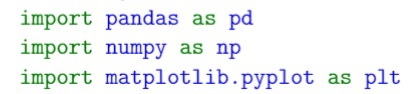
\includegraphics[height=1.6cm]{bib.jpg}
\end{center}
Para correr una celda con códigoes necesario aplicar la combinacion de las teclas \textit{Shift+Enter}, esta opción crea inmediatamente una celda abajo para seguir programando.

\subsection{Comandos}
\subsubsection{Lectura de Documento}
Digamos que queremos leer el documento de \textit{Chínipas de Almada, Chihuahua}, el código para hacerlo seria de la suiguiente manera:\\

\begin{center}
	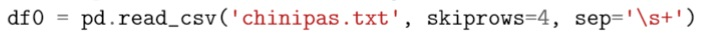
\includegraphics[height=0.5cm]{leer.jpg}
\end{center}
 Esto es posible mediante Pandas, debemos nombrar con una variable el documento que guarda la información, se sigue de un igual y la refrencia de lectura con Pandas, el nombre del documento y la información o encabezados que nos debemos de saltar del documento (por lo regular antes de los datos vienen encabezados).\\
 
 Para poder imprimir datos leídos del documento es necesario utilizar la función \textit{head()}, que si es usada así tal cual imprime las primeras 5 lineas pero si colocamos en el paréntesis un número entero n, esas n lineas imprimirá.\\
 
 Como ejemplo las primeras 5 lineas del documento:
 \begin{center}
	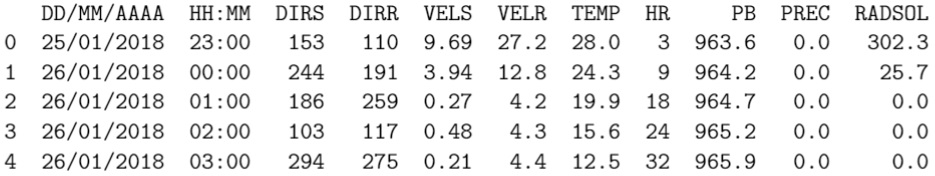
\includegraphics[height=3cm]{head.jpg}
\end{center}
\subsubsection{Estructura y Tipo de Datos}
Con Pandas podemos hacer que se acomoden los textos a leer por Phyton, ya que no se saben que estructura guardan. Por lo que se utiliza una función y se crea una varibale que guarde los datos y la estructura. 
La función quedaría de la siguiente manera:
 \begin{center}
	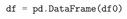
\includegraphics[height=0.7cm]{data.jpg}
\end{center}
Para saber que tipo de datos esta leyendo pandas, podemos hacer uso de la siguiente función y nos despliega la tabla de acontinuación:
 \begin{center}
	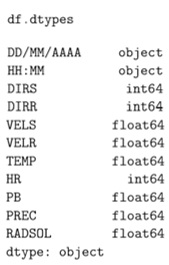
\includegraphics[height=5cm]{tipes.jpg}
\end{center}
\subsubsection{Mezclar y Eliminar Columnas}
Para mezclar la información de columnas y crear una nueva con los datos, se utilizó la siguiente función con nuestro ejemplo:
 \begin{center}
	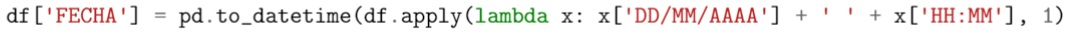
\includegraphics[height=0.5cm]{mez.jpg}
\end{center}
Donde FECHA será la nueva columna en la que se mezclaran fecha y hora.\\
Para el caso de eliminación se ocupa la siguiente función:
 \begin{center}
	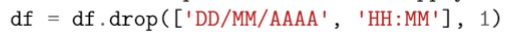
\includegraphics[height=0.5cm]{el.jpg}
\end{center}
Donde eliminaremos la fecha y lo hora.

\subsubsection{Análisis Exploratorio de Datos}
El análisis exploratorio de datos, ofrece una tabla en la que se muestran una descripción cantitativa con la mucha o poca cantidad de datos del documento,es decir, nos muestra la media, estándar, los cuartiles, la mínima y máxima de ada columna. Se obtien con la función siguiente, se muestra el ejemplo para el documento que estamos tratando:
 \begin{center}
	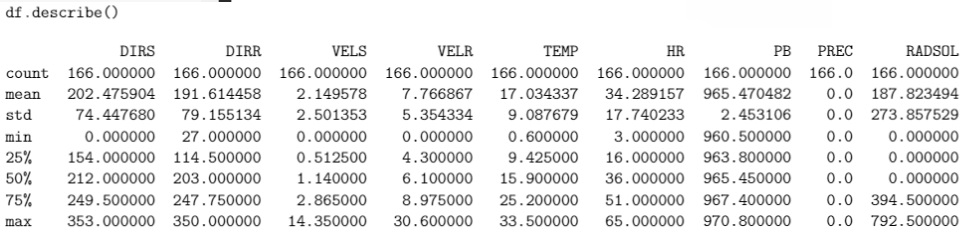
\includegraphics[height=4cm]{expl.jpg}
\end{center}

\subsubsection{Datos Condicionados en Tabla}
Para mostar ciertos datos en una tabla, es decir, condicionar datos. se hace uso de lo siguiente, haciendo seguimiento con nuestro documento:
\begin{center}
	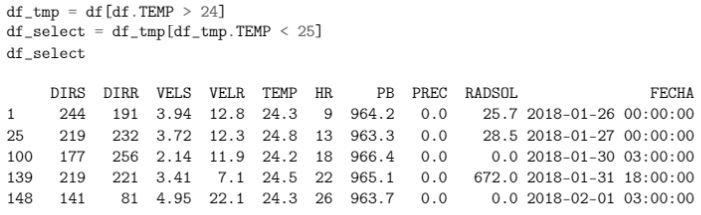
\includegraphics[height=4cm]{condi.jpg}
\end{center}
Como se puede notar estamos presentando una tabla con valores de temperatura entre cierto rango.
\subsubsection{Valores Promedio}
Si queremos conocer el valor promedio de los datos, recurrimos a la función que acontinuación se presentará y nos dará el promedio por cada columna. En el ejemplo quedaron de la siguiente manera:
\begin{center}
	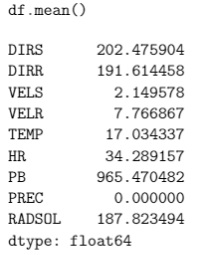
\includegraphics[height=4cm]{prom.jpg}           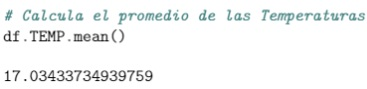
\includegraphics[height=2cm]{prom1.jpg}
\end{center}
\subsection{Graficación}
Con el paquete de matplotlib podemos crear diversas graficas. Donde ejemplo de un código de ellas es el siguiente:
\begin{center}
	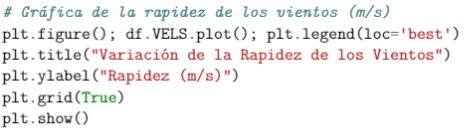
\includegraphics[height=3cm]{rap.jpg}
\end{center}
Donde figure indica la realización de una gráfica, df.VELS.plot es lo que se va a graficar, plt.legend hrá que las leyendas se acomoden donde mejor parezcan, title, ylabel y xlabes son el titulo de la gráfica y sus ejes, grid muestra la cuadrícula y plt.show() imprime. La gráfica del código anterior es la siguiente:
\begin{center}
	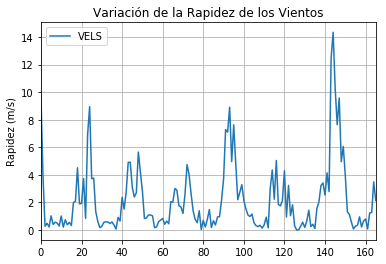
\includegraphics[height=5cm]{output_11_0.png}
\end{center}
Ahora bien, para tener dos valores en una misma gráfica tenemos como ejemplo lo siguiente:
\begin{center}
	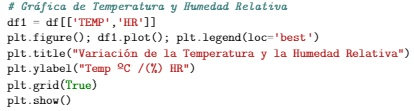
\includegraphics[height=3cm]{th.jpg}
\end{center}
\begin{center}
	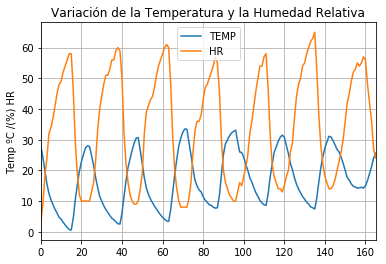
\includegraphics[height=5cm]{output_12_1.png}
\end{center}
Aquí podemos notar que mientras más humedad exista, menor sera la temperatura.\\

Seguiendo con los ejemplos de nuestro Documento, se nos pidió que hicieramos las siguientes gráficas:
\begin{center}
	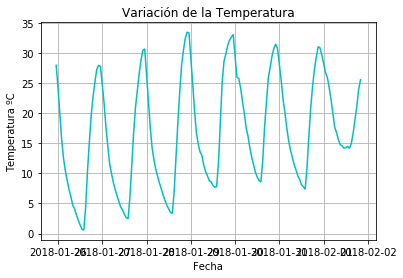
\includegraphics[height=5cm]{output_13_0.png}
\end{center}
Que nos muestra como cambia la temperatura a través del tiempo. (De los días en los que se tomó la muestra de datos).\\

A continuación se muestran las gráficas de la rápidez de los vientos y de las ráfagas, tenemos a la izquierda la general (de todos los datos del documento). Y a la derecha una particular (de datos tomados en un solo día), cabe resaltar que las horas en ésta estan transformadas, ya que los datos son tomados desde hora central, por lo que las 07:00:00 hr de nuestro horario, son las 00:00:00 hr de la hora central.
\begin{center}
	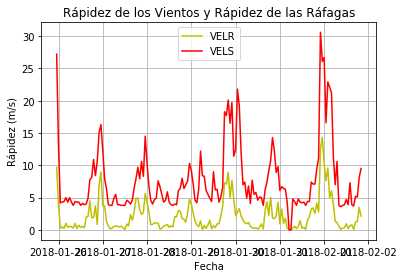
\includegraphics[height=5cm]{output_14_0.png}
    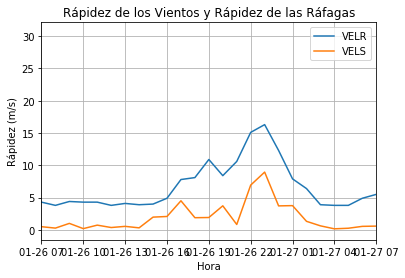
\includegraphics[height=5cm]{output_15_0.png}
\end{center}
Podemos rescatar de la gráfica de la derecha que las horas del día en las que tenemos más vientos es desde las 12:00:00 hrs hasta las 18:00:00 hrs medidos desde nuestro sistema de referencia.\\

La siguiente gráfica muestra la dirección de los vientos a lo largo de que transcurre el tiempo:
\begin{center}
	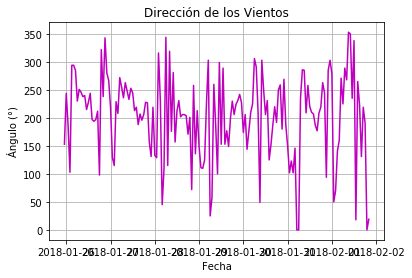
\includegraphics[height=5cm]{output_16_0.png}
\end{center}
Notando que los vientos dominantes andan en un promedio de 200 $^\circ$\\

En cuanto a la radiación solar tenemos las siguientes gráficas, a la izquierda la general y a la derecha la de un día en específico:
\begin{center}
	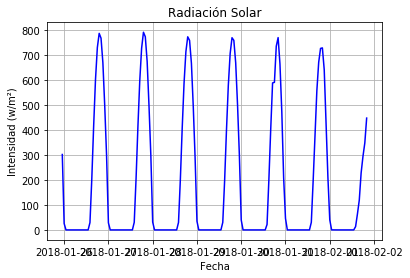
\includegraphics[height=5cm]{output_17_0.png}
    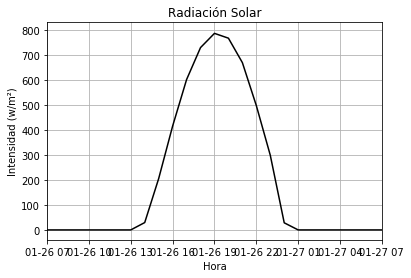
\includegraphics[height=5cm]{output_18_0.png}
\end{center}
Agregando que según nuestro sistema de referencia las horas del día con mas radiación solar son a mediodía, ya que el Sol se encuentra paralelo a los detectores y es por ello que marca mas radiación.\\

También se nos pidió que calcularamos la diferencia de temperaturas entre la máxima y la mínima de un día, y el resultado con su respecto código es el siguiente:
\begin{center}
	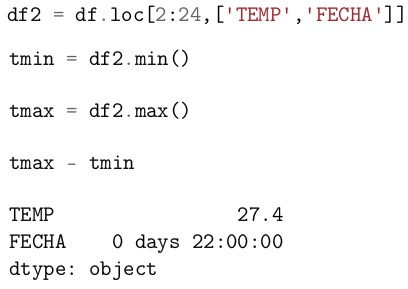
\includegraphics[height=5cm]{tempe.png}
\end{center}
Por último se realizó un análisis exploratorio de datos y el resultado fue el siguiente:
\begin{center}
	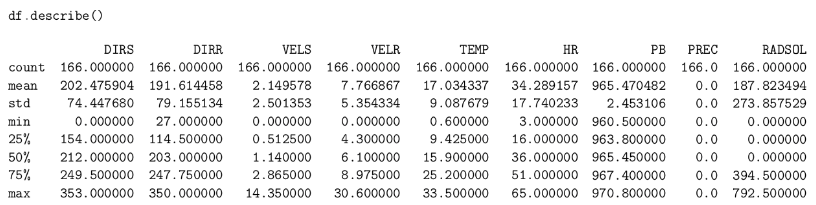
\includegraphics[height=4cm]{df.png}
\end{center}
Con esto se finalizó la actividad, a lo que podemos llamar la primera interacción con el lenguaje de programación Python, el uso de Jupyter Notebook y todas las bibliotecas.

\section{Conclusión}
A manera de conclusión de esta práctica puedo decir que fue bastante conocimiento básico el que se adquirió con el desarrollo de las actividades planteadas, procurando mas retroalimentación en las siguientes.\\

El hecho de trabajar con datos proporcionados con el Servicio Meteorlógico Nacional, nos hace reflexionar de la multidisciplinariedad de la Física.

\section{Apéndice}
\begin{enumerate}
\item ¿Cuál es tu primera impresión de Jupyter Notebook?\\

\textit{En un principio pensé que jamas iba a poder llegar a saber, pues lo veía muy complicado y más aún por que mi inglés no es muy bueno, pero con el desarrolo de actividades fui comprendiendo y me parece muy padre.}

\item  ¿Se te dificultó leer código en Python?\\

\textit{Sí, la verdad me fue muy difícil comprender ciertas partes de código, pero con lecturas e investigación logré poder modificar e incluso generar nuevo código para la actividad.}

\item  ¿En base a tu experiencia de programación en Fortran, que te parece el entorno de trabajar en Python?\\

\textit{Se ve muy bien, pareciera que Python es de mejor manejo (por ahora), pero si difiere mucho con el código a usar con Fortran.}

\item  A diferencia de Fortran, ahora se producen las gráficas utilizando la biblioteca Matplotlib. ¿Cómo fue tu experiencia?. \\

\textit{Me gustó mucho poder ver las gráficas y la manera rápida y sencilla de crearlas y modificarlas. Con Fortran no me quedaron muy en claro el uso para la graficación.}

\item En general, ¿qué te pereció el entorno de trabajo en Python? \\

\textit{Muy padre, espero con el desarrollo de las demás actividades poder lograr "dominar" este lenguaje. Espero mucho de él.}

\item  ¿Qué opinas de la actividad? ¿Estuvo compleja? ¿Mucho material nuevo? ¿Que le faltó o que le sobró? ¿Qué modificarías para mejorar? \\

\textit{La actividad en sí me gusto mucho, trabajar con datos me gusta, ya que de alguna u otra manera logras inferir buenas conclusiones de ellos. No estuvo dificil, quiza en un principio si, pero despues se fueron complementando y entendiendo las cosas. Si fue material nuevo pero se logró entender, creo que fue muy completa.}

\item ¿Comentarios adicionales que desees compartir? \\

\textit{La verdad estoy muy contento con aprender este nuevo lenguaje.}
\end{enumerate}

\section{Bibliografía}
\begin{itemize}
\item Jupyter notebook: documenta y ejecuta código desde el navegador | Desde Linux. (2018). Obtenido de: 
https://blog.desdelinux.net/jupyter-notebook/
\item Jupyter: Data Science aplicada - Paradigma. (2018). obtenido de:\\
https://www.paradigmadigital.com/dev/jupyter-data-science-aplicada/
\item Guía de inicio rápido de Jupyter Notebook. (2018). Obtenido de: \\https://live.osgeo.org/es/quickstart/jupyter\_quickstart.html
\end{itemize}

\end{document}
